\documentclass[aspectratio=169, hyperref={bookmarks=false}]{beamer}
\usepackage[T2A,T1]{fontenc}
\usepackage[english, russian]{babel}
\usepackage[utf8]{inputenc}

\hypersetup{unicode=true}

\usepackage{graphicx}
\graphicspath{{Plots/PDF/}}

\usepackage[export]{adjustbox}

\setbeamertemplate{navigation symbols}{}

\title{Поверхностная фотометрия галактик}
\subtitle{Отчет по галактике UGC 1198}
\author{Павел Соболев, Александр Крыжановский}
\date{}

\begin{document}

\frame{\titlepage}

\begin{frame}
 \frametitle{Информация о галактике}
 
    \vspace{-1cm}
    Тип: эллиптическая; \\
    Наклон: видна под небольшим углом; \\
    Видимость: незаходящая; \\
    Яркость: заметно ярче в фильтре R; \\
    Прямое восхождение: $ \textit{01}^{\hspace{1pt}h} \textit{49}^{\hspace{1pt}m} \textit{17}^{\hspace{1pt}s}\hspace{-4pt}\textit{.663} $; \\
    Склонение: $ \textit{85}^{\hspace{1pt}\circ} \textit{15}^{\hspace{1pt}'} \textit{37}^{\hspace{1pt}''}\hspace{-5pt}\textit{.94} $ \par
    
    \vspace{\baselineskip}
    Также заметны два ярких элемента в центре объекта, \\
    похожие на ядра взаимодействующих галактик
 
\end{frame}


\begin{frame}
\frametitle{Обработанное изображение, фильтр B}

    \begin{minipage}[h]{\linewidth} 
    \center{\fbox{\includegraphics[trim={0 8cm 0 0}, max height=7cm,max width=7cm]{ObjectC_B}}}
    \end{minipage}

\end{frame}

\begin{frame}
\frametitle{Изофоты, фильтр B}

    \begin{minipage}[h]{0.9\linewidth} 
    \center{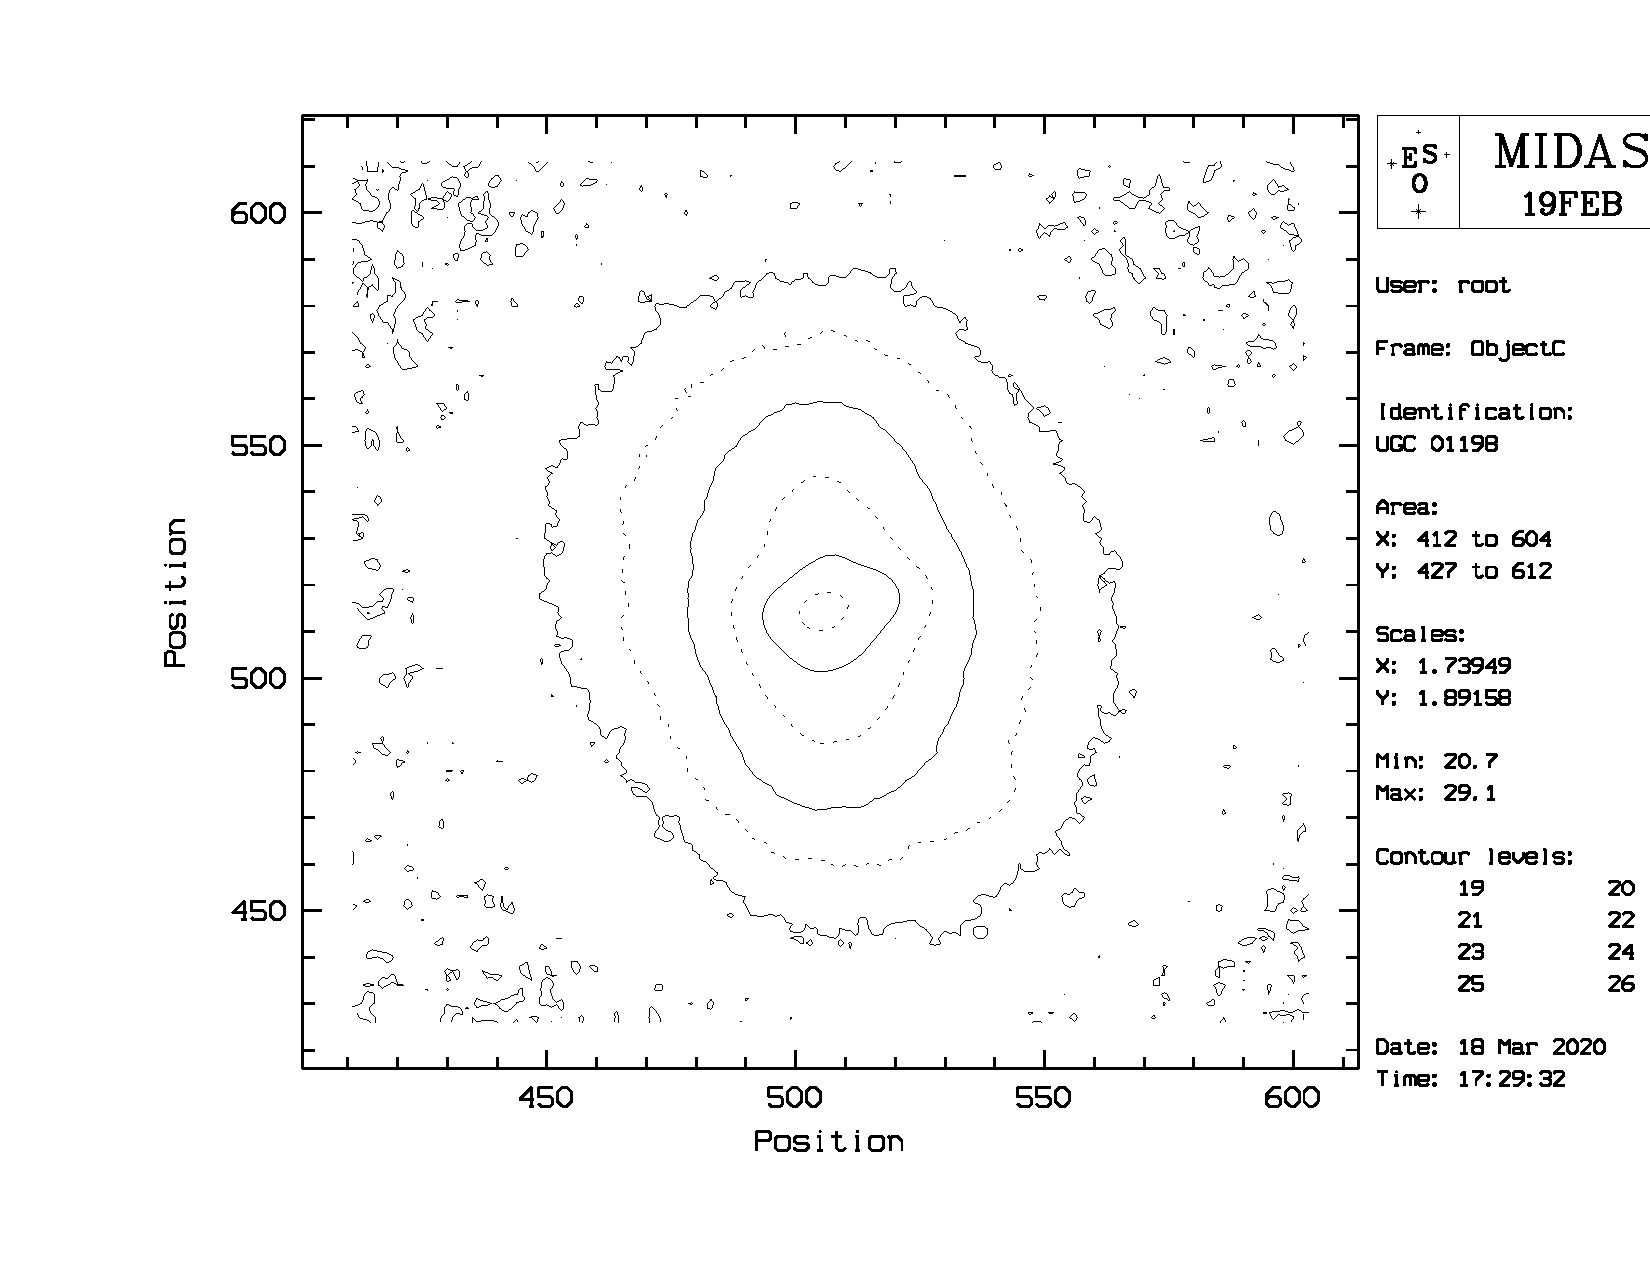
\includegraphics[totalheight=8cm]{Isophote_B}}
    \end{minipage}

\end{frame}

\begin{frame}
\frametitle{Разрезы, фильтр B}

    \begin{minipage}[h]{0.9\linewidth}
    \center{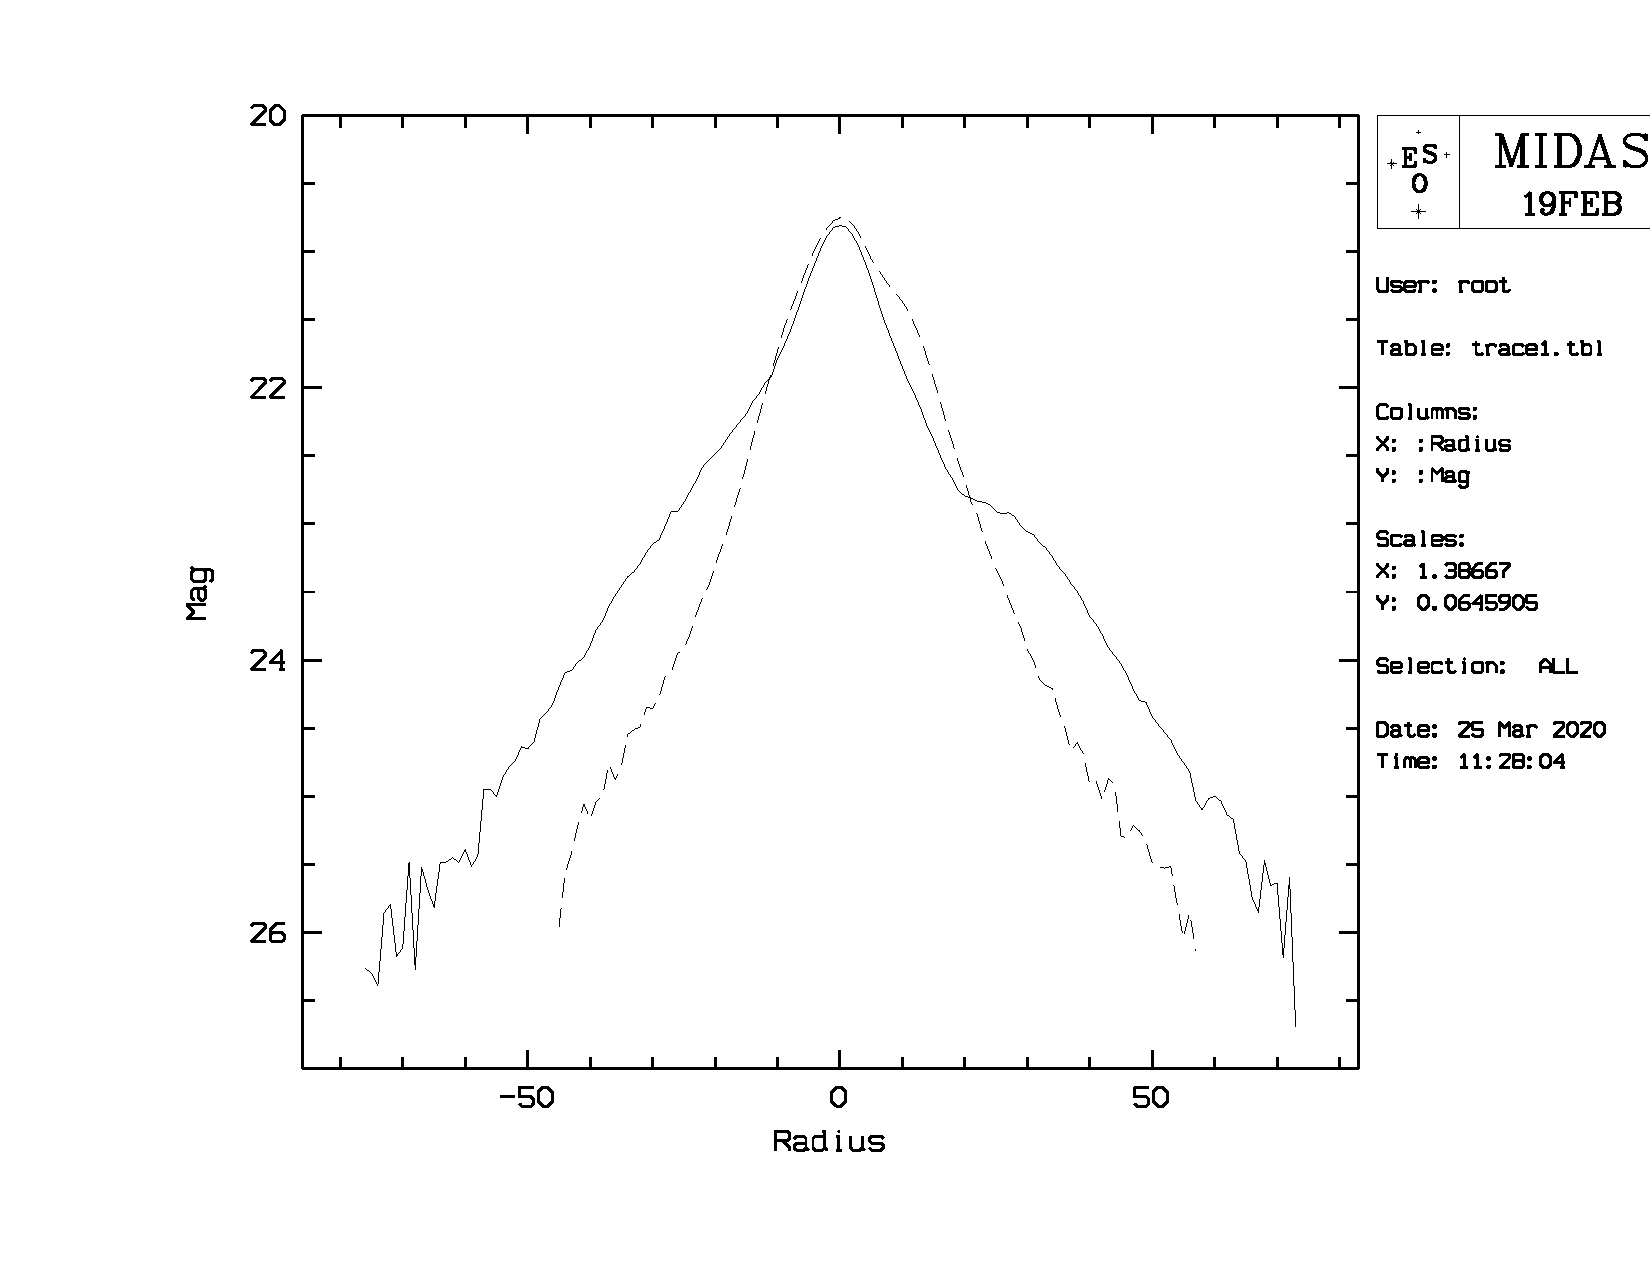
\includegraphics[totalheight=8cm]{Cuts_B}}
    \end{minipage}

\end{frame}

\begin{frame}
\frametitle{Обработанное изображение, фильтр R}

    \begin{minipage}[h]{\linewidth} 
    \center{\fbox{\includegraphics[trim={0 9cm 0 0}, max height=7cm,max width=7cm]{ObjectC_R}}}
    \end{minipage}
 
\end{frame}

\begin{frame}
\frametitle{Изофоты, фильтр R}

    \begin{minipage}[h]{0.9\linewidth} 
    \center{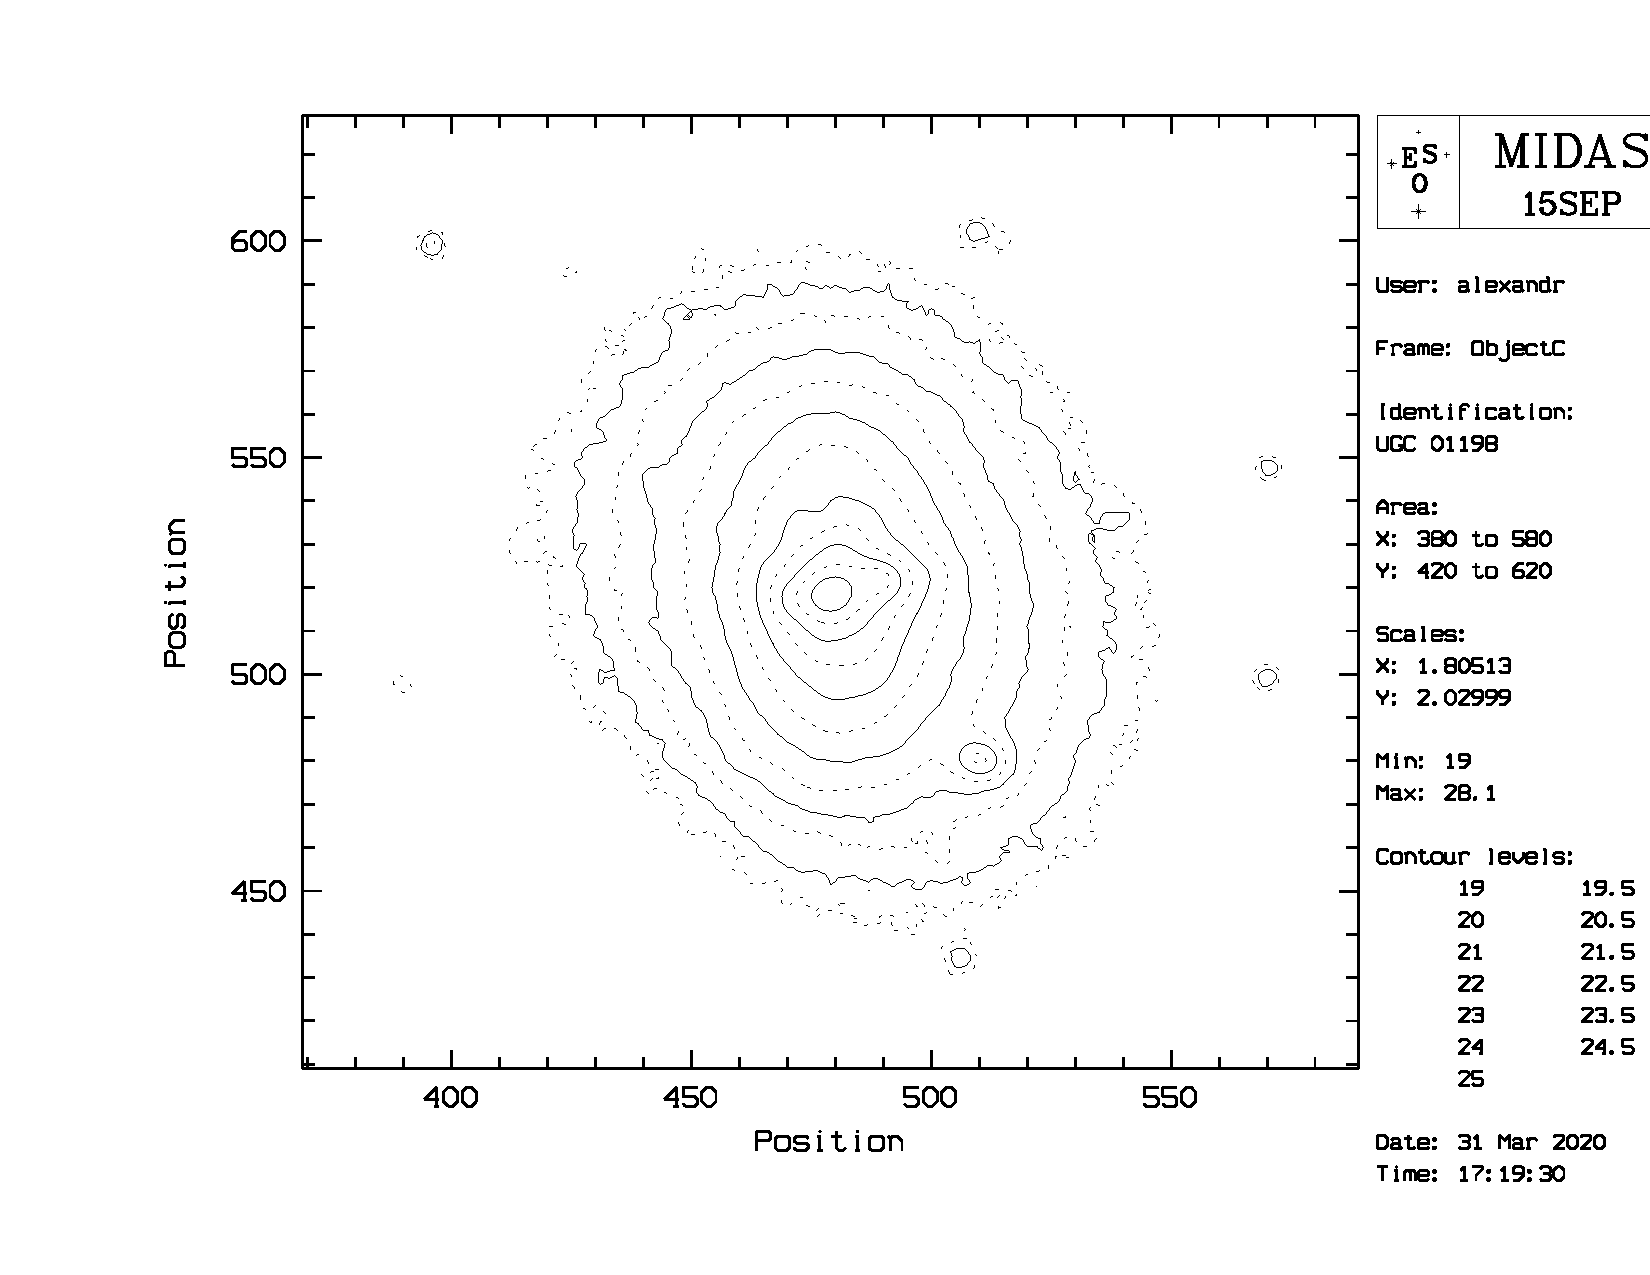
\includegraphics[totalheight=8cm]{Isophote_R}}
    \end{minipage}

\end{frame}

\begin{frame}
\frametitle{Разрезы, фильтр R}

    \begin{minipage}[h]{0.9\linewidth}
    \center{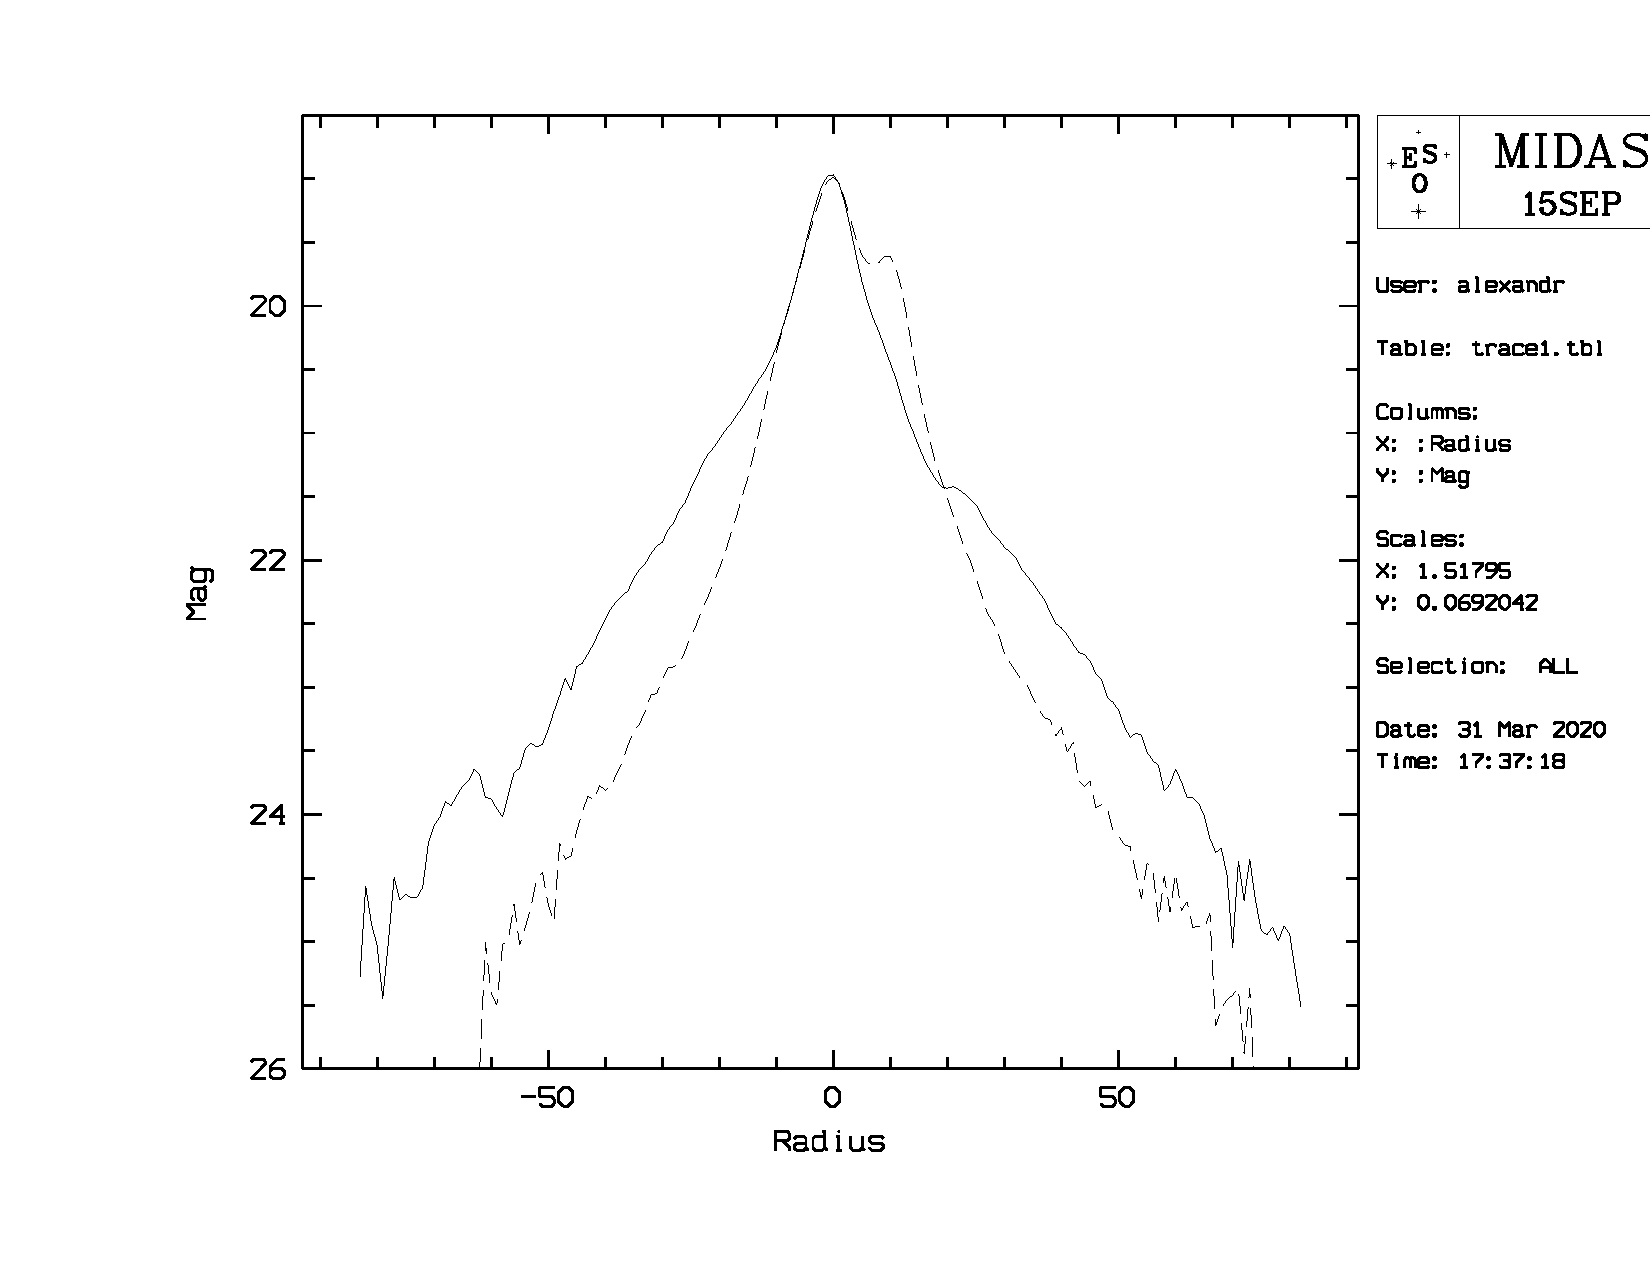
\includegraphics[totalheight=8cm]{Cuts_R}}
    \end{minipage}

\end{frame}

\end{document}
